\subsection{Rule Offload}
\label{s:offload}

\begin{figure}
\centering
%\begin{minipage}{.45\textwidth}
  \centering
  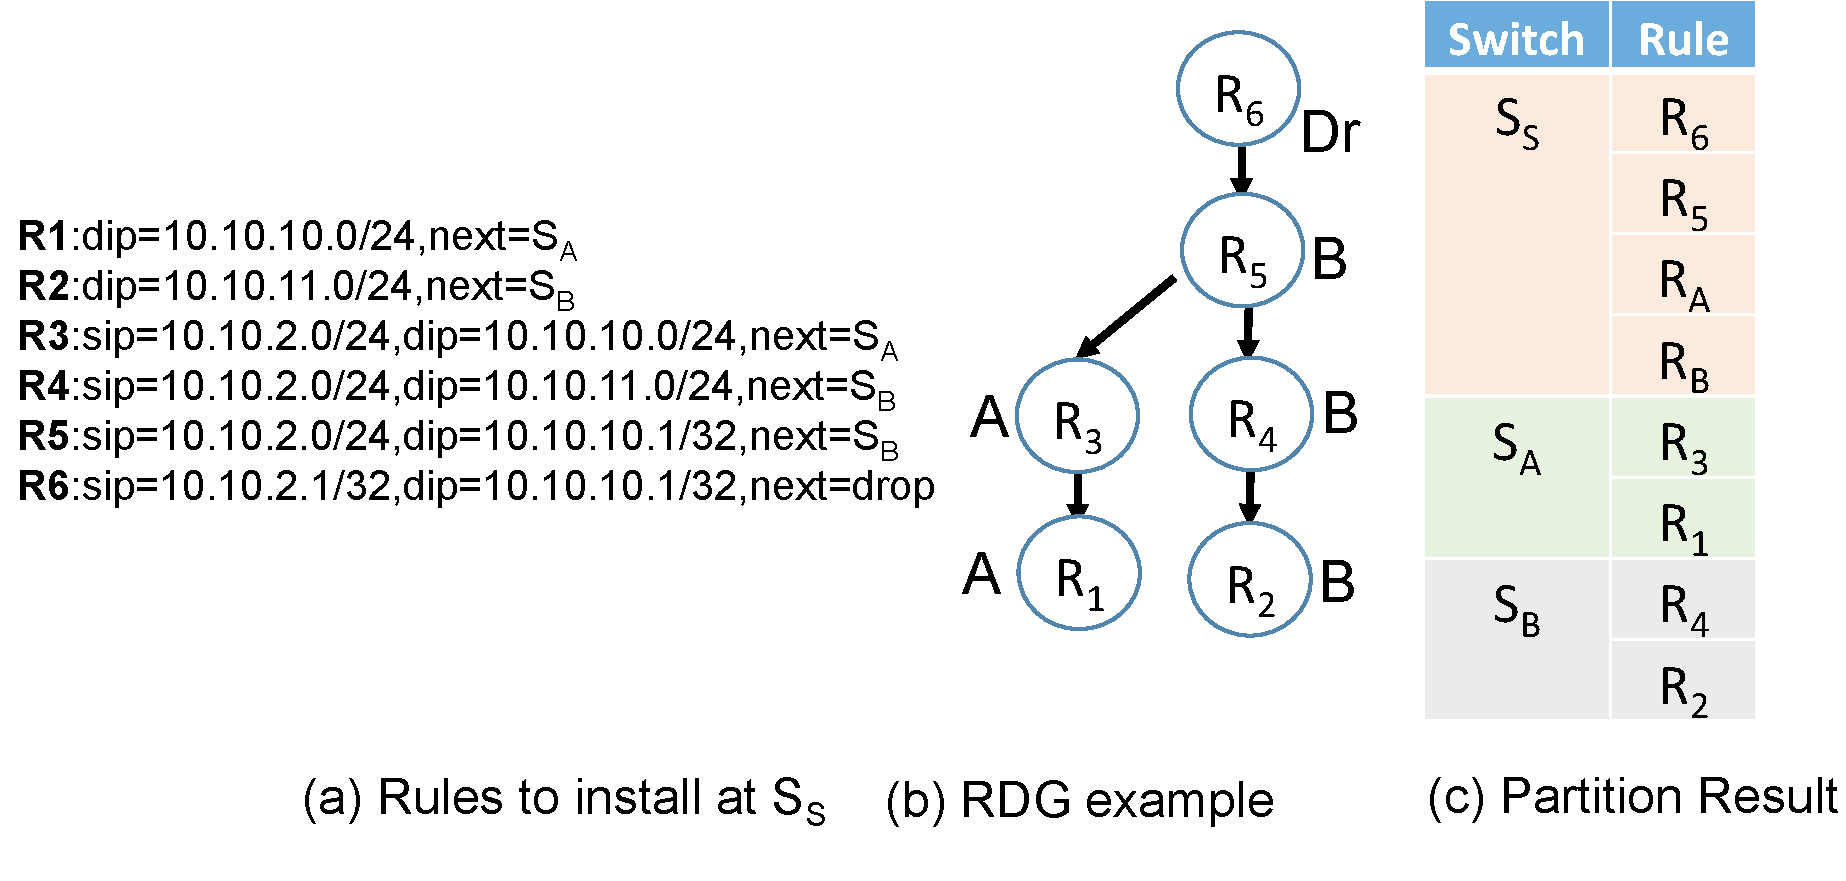
\includegraphics[width=3.0in]{figs/Rule-Offload2.pdf}
\compactcaption{Rule offloading example}
\label{fig:rule-offload}
\end{figure}

%\aditya{LI: this section does not talk about differences wrt difane, vcrib. li, can you fix?}
%\aditya{LI: we should also talk about encapsulation on the core router}

Rule offloading applies particularly to networks where tunnels are
used, e.g., cellular networks (\S\ref{sec-motivation}), carrier networks
that rely on label-switching, data centers using VXLAN
%~\cite{xxx} \aditya{check this} 
and inter-DC WAN networks such as those considered
in~\cite{swan,b4}. In such networks, SDN applications
control the tunnel end-points to setup overlay paths. Compared to the rate of
changes at these tunnel end-points, the underlay, which may also be
run using an SDN, maintains much smaller forwarding state, and
observes much less churn in forwarding state. {\em Our approach
  leverages these attributes of switches in the underlay to offload to
  them rules that would otherwise be installed at the tunnel end
  points.} 

Thus, we wish to partition rules to be installed into a switch into
subsets that can be installed at downstream switches, with the appropriate
default rules added at upstream switches. If the original number of rules is $N$
and no partition (together with default rules) has more than $H$ rules, then we can
reduce rule installation latency by a factor of $\frac{N}{H}$ by updating the
partitions in parallel. 

The main idea in our algorithm is to recursively partition the rules into a
number of child partitions. Since we offload to next hop switches, each
partition has an associated next hop. Rules in
the same partition all go to the same next hop.   
%Actions of rules in a child partition go to the same
%next hop. \aditya{prev sentence does not parse} 
The partition algorithm ensures that there is no dependency among child
partitions. For each partition, we also compute default rules to
direct packets to that partition. The objective is to maximize the number of
rules that can be offloaded minus the number of default rules introduced. 

%li: do not want to disrupt the flow by adding DIFANE; they can read that in
%related work!
%decided the delete the following
\iffalse
Different from~\cite{minlanvcrib}'s goal of reducing computational
load of host hypervisor, our goal in rule offloading is to reduce path
setup latency by enabling fast parallel execution of updates. Also, per
source rule offloading is considered in~\cite{minlanvcrib}. In
contrast, we offload by grouping the next hop of rule actions to
increase offloading opportunities. 
\fi

\fixme{re-present rule offloading}

Before calculating the child partitions, 
we first represent the rules to be installed at the tunnel 
end-point as a rule dependency graph (RDG).  
In a RDG, a node denotes a rule, an edge represents 
the dependency between two rules and the label for 
each node represents the action (or next hop) of the rule. 
%\li{add two simple examples: one for a two-node topology, one for a three-node
%star topology }
We illustrate this using an example in
Figure~\ref{fig:rule-offload}. Figure~\ref{fig:rule-offload}(a) shows the 
topology. Suppose we need to install six rules $R_1$, $R_2$,$\cdots$,$R_6$ to
switch $S_1$. The rule dependency graph is shown in Figure~\ref{fig:rule-offload}(b).
%li: add how to handle rules in table
%If there are rule entries in the flow table, the dependency graph will include
%those rules. 
For example, there is an edge from $R_3$ to
$R_1$. This means that the two rules overlap. When a packet matches both rules,
$R_3$ takes precedence. The labels $A$ and $B$ denote the next hop of the
rules' action. If a rule's action is to send through a tunnel, the label will be
the next hop of the tunnel path, not the tunnel destination.  If a rule's action
is deny, for simplicity, it will not be offloaded. The pseudo code is 
described in Algorithm~\ref{alg:partition}. The time complexity of this algorithm is 
 $\mathcal{O}$($\abs{V}$+$\abs{E}$), where $V$ and $E$ are the 
vertex and edges of rule dependency graph $G$. 
%we can handle the rule depending on the policy and the flow space
%matching it. If it 
%depending on policies, the rule can be skipped in the offloading
%algorithm or can be assigned any next hop. 
%\aditya{this seems wrong; deny rules should apply to *all* paths?} 
%It will be easy to handle deny
%rules. For simplicity, we only consider accept rules. 

\begin{algorithm}
 \KwData{$G$: RDG with nodes annotated with next hop label, 
	$H$: a bound of rule count for core switches,
	$H_{core}$: the maximum number of rules any edge switch 
           can offload to a core switch}
 \KwResult{$P$: partition set for next hops, initially empty}
  \tcc{traverse reverse edges}
  %$N$ = min($H$, $H\_core$)\;
  $G'$ = reverse($G$)\; 
 \While{BFS from leaf node of $G'$}{
  \tcc{$R$ is the current node}
  $i$ = label($R$)\;
  \uIf{$R$ depends on no other rules}{
	 \uIf{rule count of $P_i > H_{core}$ \em{or} core switch $i$'s
	 total rule count $>H$} {
		pin $R$ to $P_{root}$\;
         }
         \Else{
   	       include $R$ in partition $P_i$;\
	 }
   }
   \tcc{$R$ depends on rules with more than one distinct label}
   \Else{
       pin $R$ to $P_{root}$\;
   }
 }
 \caption{Rule Partition}
 \label{alg:partition}
\end{algorithm}

The algorithm starts from the leaf nodes (rules $R$ such that there is no $R'$ with
$R \rightarrow R'$). All of them with the same next hop are placed in one
partition. 
The outcome of the above routine is an allocation of rules to the root
(ingress switch), and to its next hops.
%try to make the following simpler
\iffalse
In the example, we have two next hops $S_3$ and $S_2$ through port A
and B respectively. We have two leaf rules $R_1$ and $R_2$. $R_1$'s next hop is
$S_3$ and $R_2$'s next hop is $S_2$. $R_1$ will be in partition 1 and $R_2$ will
be in partition 2. Since we have $R_3 \rightarrow R_1$ and $R_3$'s next hop is
the same as $R_1$ (which is $S_3$ through port $A$), and $R_2$ (nexthop $S_2$)
and R3 have no dependency, then $R_3$ will be in partition 1. Similarly, $R_4$
will be in partition 2. For $R_5$, $R_5 \rightarrow R_3$, and $R_5 \rightarrow
R_4$; thus, $R_5$ has to be in the root partition (``pinned'' to the ingress switch
$S_1$). Also all rules $R'$ such that $R' \rightarrow R_5$ will be pinned down in
a similar fashion. $R_6$ is such a rule. So $R_6$ will be in the root
partition.
\fi
In the example, we have two next hops $S_3$ and $S_2$ through port A
and B respectively. $R_1$ will be in partition 1 and $R_2$ will
be in partition 2. Since we have $R_3 \rightarrow R_1$ and $R_3$'s next hop is
the same as $R_1$, then $R_3$ will be in partition 1. Similarly, $R_4$
will be in partition 2. $R_5$ has to be in the root partition becase it has dependencies. 
Also all rules $R'$ such that $R' \rightarrow R_5$ will be pinned down in
a similar fashion. $R_6$ is such a rule. So $R_6$ will be in the root
partition.
Because we need to direct
traffic to the appropriate next hop for offloading, we need to create default
rules to cover the flowspace of the partitions (we will explain later). 
Suppose one rule $R_A$ covers
the flowspace of partition 1 and one rule $R_B$ covers the flowspace of
partition 2. The final rules to install at switches $S_1,S_2,S_3$ is shown in
Figure~\ref{fig:rule-offload}(c). Four rules will be installed in switch $S_1$
and two each will be installed at switches $S_2,S_3$ respectively. This reduces
the number of rules to install at switch $R_1$ by one third.

We start by picking a bound $H<N$ for the rules at any switch, where $N$ is the
total number of rules we started with that were to be installed at the edge
switch. We also use a bound $H_{core}$ that controls the maximum number of rules
{\em any} edge switch can offload to a given core switch. If at any iteration,
partitioning at a node causes either of these bounds to be violated at a
downstream core switch, then we terminate partitioning for the node. 


We then run the above routine recursively starting at the edge switch,
followed by running it at the next hop core switches over the rules
allocated to them, and so on. The termination condition is that a set
number of next hops (downstream switches in the tree rooted at the
edge switch) are explored. If at termination, the number of rules
accommodated at every core switch is $<H$, then we lower $H$ by a factor
$\gamma < 1$ and repeat again. If $H^*$ is the value of $H$ at the last of
such iterations, then we achieve a speedup of $\frac{N}{H^*}$ from
installing the offload rules in parallel. When running this scheme across the network, 
we sort edge nodes in
decreasing order of rules to be installed and run the above algorithm
on them in this order. In our algorithom, we assume that all the switches
have the same latency model for simplicity. 
To accommodate switch diversity, 
we can assign different cost for the rules offloaded to different core switches.

\iffalse
For ease of description, in the above algorithm, we do not account for switch
table occupancy or consider the detailed delay model as in
Section~\ref{s:floweng}. To accommodate table occupancy, we can stop rule
offloading process on a particular switch if the occupancy level will exceed a
threshold. To avoid high delays due to rule structure in core switches, we apply
the detailed delay model to our partition results. If the estimated delay is
higher than no offloading because of a particular core switch, we will remove
that switch from consideration and rerun the algorithm. It is also easy to
consider the delay model directly in our algorithm as we have done for flow
engineering in Section~\ref{s:floweng}. However, for simplicity, we omit the
details. 
\fi


\iffalse
\program{prog:rule-offload}
    {Recursive Rule Partition Algorithm}
{
//G: rule dependency graph with nodes annotated with next hop label \\
//$\mathcal{P}_i$: partition $i$ for next hop $i$, initially empty \\
//$C_i$: set of rules covering the flowspace of partition $i$ \\
//$N$: threshold for extra covering rules  \\
While (BFS from leaf node) \{ //traverse reverse edges\\
\> If rule $R_i$ with label $L_i$ depends on no other rules, \\
\>\>\> include $R_i$ in $\mathcal{P}_{L_i}$\\ 
\> Else If rule $R_i$ depends on rules with more than one distinct label \\
\>\>\> pin the rule to the root partition \\
\> Else \\ 
\>\>\> If rule $R_i$ results in $n>N$ covering rules, \\
\>\>\>\>\>\>    skip $R_i$ \\
\>\>\> Else     include $R_i$ in $\mathcal{P}_{L_i}$\\ 
\} \\
}
\fi

%Partition algorithm:
%We assume for simplicity there are two next hops at every switch. This can be
%easily generalized where there are $k_s$ next hops at switch s. 
%This algorithm is run first at ingress over entire rule set.
%Once rules are spread out as above we need to specify default rules. 
%Lwts look at  default rule creation algorithm. One possibility: 

%\li{What is the default rule maintainence algorithm?}

\iffalse

We conclude by describing how to compute default rules. Specifically, given two
partitions A and B computed above, we wish to determine default rules that need
to go into A and B's root partition. The main challenge is dealing with the fact
that the simplistic default rules described above may have a non-empty
intersection, where the intersection has rules from either A or B. This
introduces ambiguity at the root. Splitting up the default rules into smaller
parts to try and deal with this may introduce too may default rules. We present
a heuristic optimization. 

We assume that each rule can be represented by a rectangle (src  IP range, dst
IP range) for simplicity. Our heuristic below can be easily extended to higher
dimensions. The key idea is, given the rules in A and B, we divide the
address range into halves; each half is called a region. 

We check if the ratio of rules in \textit{max}(|A|,|B|) to (|A| + |B|) is above
some threshold $\Theta$ in a region. If so, we create one default rule for
\textit{max}(|A|,|B|) and install it in the root. Furthermore, we "promote" all
the rules of the other partition to root and pin them there. 

If, however, the number of rules in  \textit{max}(|A|,|B|) to (|A| + |B|)  below
$\Theta$ in a region and there is no rule spanning two halves of the region,
then we further divide that region in sub-regions. We repeat the process above
for each sub region. We recursively repeated this process for a small number of
step. If at the end of these steps, the combined number of default rules and
pinned rules to be installed at the root is significant ($> \Omega$), then we
merge A and B and simply install all of it in the root. 

\fi

{\bf Computing default rules:} Given two partitions A and B computed above, we wish determine default rules that need to go into A and B's root 
partition. The main challenge is dealing with the fact that the intersection
of default rules may have rules from either A or B. This 
introduces ambiguity at the root. Splitting up the default rules into smaller parts to try and deal with this may introduce too may default rules. We 
present a heuristic optimization, described briefly below.

We assume that each rule can be represented by a rectangle (src IP, dst IP) for simplicity. Our heuristic below can be easily extended to higher 
dimensions. Given the rules in A and B, we create {\em covering rectangles} one each for the rules in A and B, called $C_A$ and $C_B$. A covering 
rectangle is one whose src IP range covers the entire src IP range specified in the rules (likewise for destination IPs).
The pseudo code is shown in Algorithm~\ref{alg:default_rule}.
\iffalse
We check if the number of rules from either A or B in $C_A\cap C_B$ is below some threshold $\Theta$. If so, all such rules are ``promoted'' to the 
root partition and get pinned there. Furthermore, we create two default rules, one each for $C_A$ and $C_B$ and install them in the root.

If, however, the number of rules in $C_A\cap C_B$ exceeds $\Theta$, then we further divide $C_A$ and $C_B$ in two sub-rectangles each. We repeat the 
process above for pairs of sub-rectangles one corresponding to A and the other to B.
\fi


\begin{algorithm}
 \KwData{rule partition set $P$}
 \KwResult{default rules at root and new partition set $P$}
  \SetKwFunction{proc}{proc}
  $P'$ = $P$ - $P_{root}$\;
 \For{each distinct partition pair $(A, B) \in P'$}{
  get covering rectangles $C_A$ and $C_B$ for $A$ and $B$\;
  \proc{$P$, $C_A$, $C_B$}\;
  }
  \SetKwProg{myproc}{Procedure}{}{}
  \myproc{\proc{$P$, $C_A$, $C_B$}} { 
  \uIf{ rule count in $C_A$ $\cap$ $C_B$ $\geq$ $\Theta$} {
   	divide $C_A$ and $C_B$ into two sub-rectangles each\;
	\For{each sub-rectangles pair ($C'_A$, $C'_B$)}{
		\proc{$P$, $C'_A$, $C'_B$}\;
	}
	
   }
   \Else{
        move $C_A$ $\cap$ $C_B$ to $P_{root}$\;
	assign partition $A$ and $B$'s default rule as $C_A$ and $C_B$\;
   }
  }
 \caption{Computing default rules}
 \label{alg:default_rule}
\end{algorithm}

We recursively repeated this process for a small number of steps. If at the end of these steps, the combined number of default rules and pinned rules 
to be installed at the root is significant ($> \Omega$), then we merge A and B and simply install all of it at the root.

%\aditya{check this. we also need to talk about the constants chosen}

% L: Check the number of rules from either A or B that are in the intersection of $C_A$ and $C_B$.

% If this number  is less than a threshold the partition 
% 	rules in the intersection getting pinned to root
% 	two default rules are set one for each rectangle

% else 
% split the covering rectangles half way
% go to ``L'' and repeat what follows for these composite rectangles.

% Terminate splitting after some number of step. Also keep track of maximizing
% offload while minimizing default rules. 


\iffalse
The idea is to recursively partition the rules into a number of child
partitions. actions of rules in a child partition go to the same next hop. There
is no dependency among child partitions. The partition algorithm ensures this.  
The partition is offloaded to its associated next hop. For each partition, we
also compute a number of default rules to direct packets to that partition. The
objective is to maximize the number of rules can be offloaded minus the number
of default rules introduced. 

The algorithm starts from the leaf nodes (rules without any rules depending on
them). All of them with the same next hop are placed in one partition.For
example, if we two next hops A and B. Suppose we have two leaf rules R1 and
R2. R1's next hop is A and R2's next hop is B. R1 will be in partition 1 and R2
will be in partition 2.  
If we have R1 depends on R3 and R3's next hop is the same as R1 (which is A),
and R2 (nexthop B ) does not depend on R3,then R3 will be in partition 1.  
Suppose for R4, R4 depends on R1, but R2 depends on R4, then R4 has to be in the
root partition (pined to the ingress switch). Also all rules depending on R4
will be pined down. 
\fi

% LocalWords:  VXLAN SDN hypervisor nexthop flowspace parallely prog BFS src IP
% LocalWords:  dst challanges IPs recurively
